\documentclass[article,12pt]{elsarticle}
\usepackage[spanish]{babel}
\usepackage[utf8]{inputenc}
\usepackage{amssymb}
\usepackage{flushend}
\usepackage{float}
\usepackage{anysize}
\usepackage{amsmath}
\usepackage{amsfonts}
\usepackage{dcolumn}
\usepackage{amsthm}
\usepackage{caption}
\usepackage{float}
\usepackage{subfigure}
\usepackage{graphicx}
\usepackage{lmodern}
\usepackage{booktabs}
\usepackage{color}
\usepackage{longtable}
\usepackage{rotating}
\usepackage{etoolbox}
\usepackage{comment}
\usepackage{pdflscape}
\usepackage{hyperref}
\usepackage{booktabs}
\usepackage[table,xcdraw]{xcolor}


\begin{document}

\begin{frontmatter}
    \title{Laboratorio de Electromagnetismo \\
    Práctica III\\ 
    Generador de Van de Graaff y transformación de \\ energías en eléctrica.}

    \author{Iván Bautista Alvarado$^1$ y Andrés López González$^1$} %Aquí va el nombre de los integrantes que participaron en el informe.
    \address{$^1$ Facultad de Ciencias, Universidad Nacional Autónoma de México, M\'exico CDMX.}

    \begin{abstract}

In this experiment, we explore various methods of generating and storing electrical energy, with a focus on the operation of a Van de Graaff generator and the analysis of multiple energy conversion devices, including thermocouples, solar cells, electrolytic cells, and galvanic cells. The Van de Graaff generator's electrostatic effects were tested through interactions with conductive and non-conductive materials, such as LEDs, confetti, and Franklin bells, revealing phenomena such as electrostatic polarization and charge induction when it was used in the seeds. The second part of the experiment involved measuring the potential difference produced by different energy conversion devices. Among the tested methods, solar cells demonstrated the highest efficiency in terms of energy output, followed by electrolytic and galvanic cells. Thermocouples exhibited significantly lower voltage generation, confirming their unsuitability for practical energy applications on a larger scale. The experimental results are evaluated in terms of their effectiveness, cost, and applicability, providing insights into the optimal methods for generating electrical energy under varying conditions.

    \end{abstract}


    \begin{keyword}
Van de Graaff generator
Energy conversion devices
Electrostatic phenomena
Solar cells
Thermocouples
    \end{keyword}

\end{frontmatter}

    \section*{Resumen}

En este experimento, exploramos varios métodos de generación y almacenamiento de energía eléctrica, con un enfoque en el funcionamiento de un generador Van de Graaff y el análisis de múltiples dispositivos de conversión de energía, incluidos termopares, células solares, células electrolíticas y células galvánicas. Los efectos electrostáticos del generador Van de Graaff se probaron a través de interacciones con materiales conductores y no conductores, como LED, confeti y campanas de Franklin, revelando fenómenos como la polarización electrostática y la inducción de carga cuando se utilizó en las semillas. La segunda parte del experimento implicó medir la diferencia de potencial producida por diferentes dispositivos de conversión de energía. Entre los métodos probados, las células solares demostraron la mayor eficiencia en términos de producción de energía, seguidas de las células electrolíticas y galvánicas. Los termopares exhibieron una generación de voltaje significativamente menor, lo que confirma su falta de idoneidad para aplicaciones energéticas prácticas a mayor escala. Los resultados experimentales se evalúan en términos de su efectividad, costo y aplicabilidad, proporcionando información sobre los métodos óptimos para generar energía eléctrica en diferentes condiciones.

\noindent \textit{Palabras Clave}: \textit{Palabras Clave}: Generador de Van de Graaff, Dispositivos de conversión de energía, Fenómenos electrostáticos, Celdas solares, Termopares.\\ \hline


\section{Introducción}
    Para generar y almacenar carga eléctrica se han diseñado distintos instrumentos a lo largo de la historia. En este momento nos interesa un aparato en particular que es conocido como "Generador de Van de Graaff". En honor al físico Robert. J. Van de Graaff. El funcionamiento de este generador es, en esencia, bastante simple. Tiene una banda que gira sobre un riel, y en los extremos tiene dos peines, uno de ellos hace contacto con la banda y sirve para cargarla por fricción, el otro peine no toca a la banda, únicamente sirve para inducir carga la esfera externa, pues ese peine está conectado a la esfera, y por la inducción de la banda al peine, termina cargada toda la esfera. \\
    La Campana de Franklin consiste de un soporte metálico que soporta dos campanas y enmedio un péndulo con una pequeña esfera metálica.
    Al cargarse una de las campanas van a cargar a su vez a la esfera por inducción, generando un dipolo eléctrico. Este dipolo va a reaccionar al campo eléctrico que se genera entre las campanas (por la carga que ya tienen) y van a mover al péndulo hacia una de las campanas. Al tocar la campana, como la esfera es conductora, va a hamber una redistribución de las cargas, en donde la bolita queda cargada con el signo de la campana que tocó, y será atraída hacia la campana opuesta. Este proceso debería seguir hasta que la carga se disipe en el aire.\\
    Un concepto muy importante a tener en cuenta es la \textit{energía}. A pesar de su importancia es un concepto muy abstracto. En un principio la energía se asocia al movimiento que puede producir un objeto, sin embargo, con el tiempo se han descubierto muchos tipos de energía, y no todos están asociados con el movimiento. Algunos ejemplos de esta son:
    \begin{itemize}
        \item Energía cinética
        \item Energía térmica
        \item Energía eléctrica
        \item Energía química
        \item Energía del reposo
        \item Energía nucelar
    \end{itemize}
    La energía también tiene una relación con el trabajo a partir del teorema de trabajo-energía
    \begin{equation}
        \Delta W=E
    \end{equation}
    A partir de aquí podemos decir que la energía es la capacidad de generar trabajo. O de manera más explícita, es la capacidad que un objeto tiene para generar algún cambio en el entorno. Mientras más energía almecenes, más cambios podras generar. \\
    
    A lo largo de la práctica necesitaremos varios objetos que puedan generar una diferencia de potencial. Y será útil conocer un poco de ellos.
    
    Termopar: Consta de dos metales unidos en un extremo, que al calentar el extremo en donde se unen, producen una diferencia de potencial. Esto ocurre pues al calentar el metal, se va a generar un gradiente de temperatura de un extremo del metal al otro extremo. En el extremo más caliente hay una mayor exitación de las partículas por el calor, haciendo que los electrones se muevan más libremente en esa región, hasta llegar a la parte menos caliente en donde se van a acumular. la facilidad con la que se excitan los electrones y con la que la temperatura se distribuye va a dependender del metal, por eso es necesario dos metales, pues esa diferencia va a provocar también la diferencia de potencial entre ambos metales.
     
    Celda solar: Estas celdas convierten la energía de la luz solar en energía eléctrica. Esto se debe a que la celda solar esta llena de células fotoeléctricas, que es la parte más importante de la celda.
    La luz al incidir sobre un material, le transfiere energía y libera electrones debido al exceso de energía (A esto se le conoce como efecto fotoeléctrico), las células fotoeléctricas "capturan" esos electrones para poder pasar una corriente eléctrica y generar un voltaje.
 
    Celda electrolítica: Este tipo de celdas hacen uso de energía para producir una reacción redox. Consisten generalmente en dos placas que se encuentran en un mismo medio electrolítico. Y se les induce carga opuesta para producir una electrólisis del electrolito y así poder reducir y oxidar los materiales, produciendo la reacción redox. Como esto se está produciendo gracias a una electrólisis, habrá una placa que estará rodeada de moléculas de oxígeno y otras de hidrógeno.
    Esto dependerá de la pláca que esté funcionando como ánodo y la que funcione como cátodo. Pues el ánodo va a tener a las moléculas de hidrógeno, y el cátodo tendrá a los dioxígenos.
    La reacción que tenemos se ve como:
    \begin{equation}
        2H_2O \longrightarrow 2H_2 + O_2
    \end{equation}
    Gracias a esto, podemos concluir que el cátodo estará rodeado de más moléculas, y por lo tanto se verá el burbujeo más intenso.
    
    Celda galvánica: De la misma manera que las celdas electrolíticas, aquí se produce una reacción redox, sin embargo, la principal diferencia es que en este caso, la reacción si es espontantea, y en la electrolítica no lo es. Este tipo de celdas consisten en dos electrodos de distintos materiales separados en dos recipientes, en cada recipiente hay una solución de una sal correspondiente al metal del que está hecho el electrodo. Y únicamente están conectados mediante un puente salino, que es lo que permite la reacción de reducción y oxidación. De esta manera, uno de los electrodos se convertirá en un cátodo y el otro servirá como ánodo, esto dependerá de los materiales.
\subsection{Hipótesis}
Para la primera parte, se piensa obtener la reacción de los objetos, es decir, tanto las lámparas y focos led van a poder prender al acercar la mano y al tocarlos, y el confetí va a pegarse a la mano. También la campana debería funcionar como se mencionó en la introducción, y las semillas en el aceite deberían formar una figura que corresponda al campo eléctrico, que genera la carga que se generó, en el aceite.

Para la segunda parte, esperamos obtener voltajes muy pequeños para los termopares, en comparación a las celdas galvánicas y electrolíticas. El resultado que esperamos que más voltaje registre es el de las celdas solares. Sin embargo, estas suelen caras, y en términos de efectividad-precio, creemos que las celdas electrolíticas serán la mejor opción.
\subsection{Objetivos}
Observar las interacciones del Van Der Graaff con nuestros diferentes arreglos y comparar diferentes formas de obtener energía eléctrica y verificar cuál es más efectiva.
\section{Desarrollo Experimental / Métodos}
    \subsection{Parte 1:}
    Materiales utilizados:
    \begin{itemize}
        \item 1 Refractario de copa
        \item Aceite
        \item Semillas de pasto
        \item 1 Generador Van de Graaff
        \item 2 Cables caiman-caiman
        \item Cinta adhesiva
        \item 2 Electrodos
        \item Confeti
        \item Lamparas 
        \item Focos pequeños
        \item 1 campana de Franklin
        \item 1 Caja de plástico
        \item Lámparas de led de tubo
    \end{itemize}
    Para la primera etapa, se probaron de varias maneras el generador de Van de Graaff ya tieniendo este conectado y generando corriente.

    Estando parados en la caja de plástico para evitar el paso de corriente a tierra, tomamos con una mano la bola del generador y la otra mano la acercamos al confeti, a los focos led pequeños y a las lámparas de led.

    Después, con un cable cable caiman-caiman, pegado de un extremo al generador y de otro agarrado a un soporte de la campana, le transmitimos carga a la campana de Franklin.

    Por último, vaciamos aceite en el refractario de copa, aproximadamente hasta llenar 5cm. Luego se colocaron varias semillas de manera uniforme por el refractario. Ahora pegamos el extremo de un cable caiman-caiman al generador, y el otro extremo agarrando un electrodo. El otro cable caiman-caiman lo conectamos a tierra y del otro extremo se agarró al otro electrodo. Finalmente se metieron los electrodos al refractario con aceite como se muestra en el diagrama.
    \begin{figure}
    \centering
    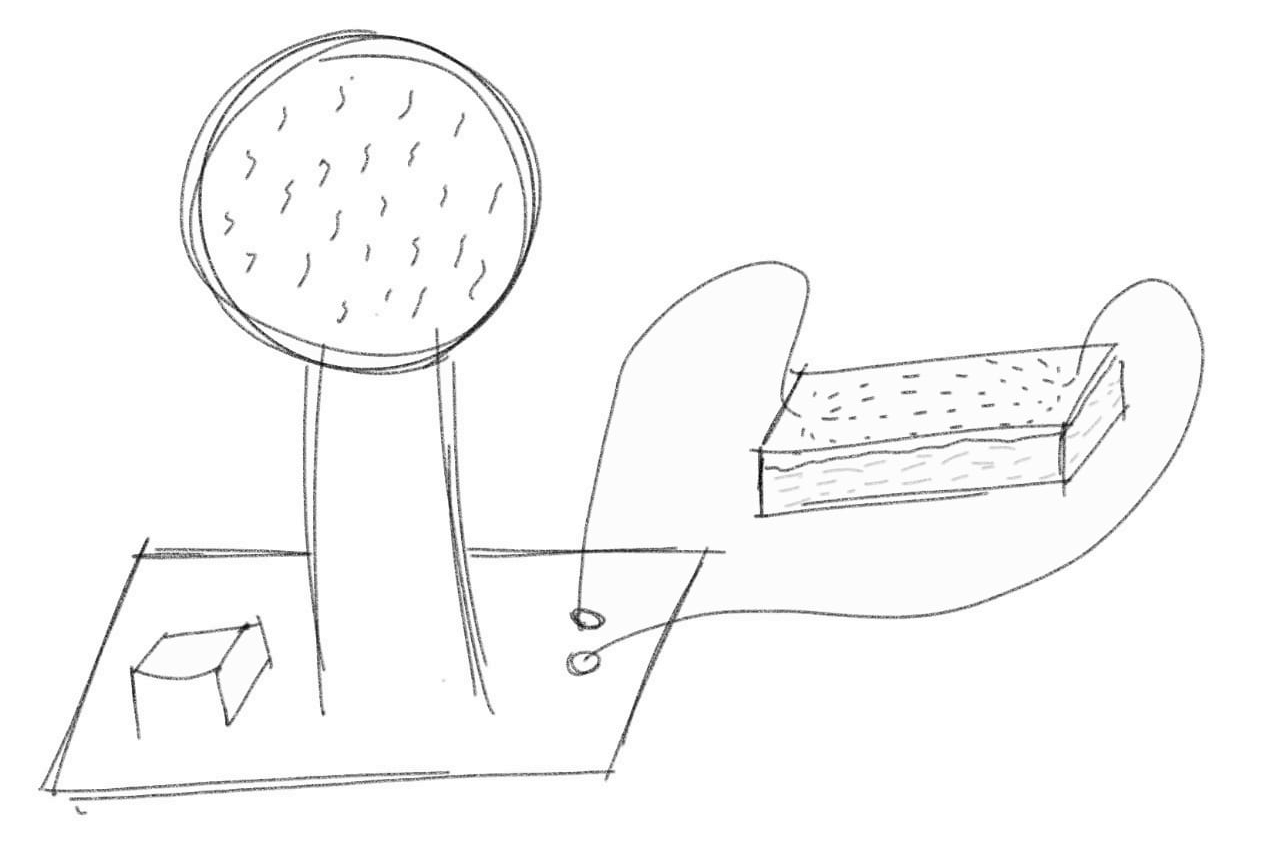
\includegraphics[width=0.5\linewidth]{vander.png}
    \caption{Van Der Graaff con semillas de pasto}
    \label{fig:enter-label}
    \end{figure}

    \subsection{Parte 2:}
    Materiales utilizados:
    \begin{itemize}
        \item 1 Multímetro
        \item 1 Pedazo de madera
        \item 1 Vela
        \item 1 vaso de precipitado de vidrio
        \item 1 lija de agua
        \item 1 Encendedor o cerillos
        \item 2 Cables banana-banana
        \item 2 Cables caiman-caiman
        \item 1 Pila de 9V
        \item 1 Celda solar
        \item 2 Frascos Gerber
        \item Vinagre
        \item Varillas de cada material: Cobre, Latón, Nicromel.
        \item 2 Laminas de cada meterial: Grafito, Lámina, Alumino, Níquel, Zinc, Latón, Estaño, Hierro, Cobre, Magnesio.
    \end{itemize}
    Para la segunda etapa se hicieron mediciones del voltaje de la siguiente manera:
    \subsubsection{Termopar}
    Se construyeron termopares con las varillas. Se tomaron dos varillas de diferente material, y se enrollaron mutuamente, de tal manera que en un extremo, sus puntas estuvieran lo mas pegadas posibles, y del otro extremo sus puntas estuvieran separadas. Es importante que no estén oxidadas las varillas, entonces, de ser necesario, se lijan los extremos de la varilla con una lija de agua\\ 
    Teniendo la vela encima del pedazo de madera, se  encendió y se acercó unicamente el extremo del termopar en donde las puntas coincidian. Ya hecho esto, con el multímetro se registra el voltaje que genera, colocando las puntas de prueba en las puntas del termopar que quedaron separadas.\\
    Esto se repitió para los pares de varillas: Cobre-Cobre, Nicromel-Latón, Cobre-Aluminio
    \subsubsection{Celda solar}
    Con la celda solar se hicieron dos diferentes mediciones de voltaje. La primera en un cuarto sin una gran entrada de luz solar, al apuntar la luz de una lámpara de un celular directamente a la celda. Para la segunda se expuso la celda a la luz solar al aire libre y se midió el voltaje.
    \subsection{Celda galvánica}
    Para esta celda usamos como electrodos una pequeña barra de zinc y otra de cobre. Cada una acomodada en su frasco de gerber, que tenía una solución de sulfato de zinc y sulfato de cobre, respectivamente a cada metal. ambos conectados por un puente salino. Con el multímetro, usando cables banana-banana con uno de los extremos conectados a una pinza caimán, se midió el voltaje, colocando cada caimán en cada placa.
    \subsubsection{Celda eletrolítica con diferentes láminas}
    Usando el vaso de precipitado de vidrio, colocamos dos láminas de los sigueintes materiales: Grafito, Lámina, Alumino, Níquel, Zinc, Latón, Estaño, Hierro, Cobre y Magnesio.  Llenamos con poco vinagre, el suficiente para que alcance a tocar a ambas láminas. Después conectamos con los cables caiman-caiman, un polo de la pila 9v a una de las lámina, y el otro polo a la otra lámina. Para medir el voltaje, sumergimos las puntas del multímetro al vinagre, cada una cerca de las láminas, pero sin tocarlas.
    Eso lo repetimos para cada par de placas, incluyendo pares iguales. y mantendiendo igual la distancia de las puntas del multímetro a las láminas.
\section{Resultados y discusión}
\subsection{Van Der Graaff}
Para nuestra primera parte con el generador de Van de Graaff, al estar un partícipe sobre una plataforma aislante y tocar el Van Der Graaff, no existieron efectos negativos a pesar de que este iba subiendo su voltaje progresivamente hasta 70V, no sentía dolor ni incomodidad, sin embargo el cabello se levantaba muy notoriamente y se separaban, esto como producto de la adquisición de cargas iguales entre los cabellos por lo que se repelían, además cuando se acercó al confeti estos se veían atraídos por la mano del partícipe, esto es debido a que a pesar que el confeti no estaba cargado ocurrieró un suceso llamado polarización electromagnética, que consiste en la redistribución de las cargas positivas y negativas en polos opuestos del material sin carga, esto provoca que una parte del material haya sido atraído con tal magnitud que haya vencido incluso la fuerza gravitacional. El otro razgo asombroso de esto es que la polarización es provocado por fuerzas a distancia que ejerce el campo electromagnético de la palma del partícipe. 
Por otra parte para focos pequeños y lámparas led largas vimos que encendieron incluso cuando apenas estaban a punto de ser tocadas, esto es debido a la carga inductiva que ejercía el partícipe y cuando la tocaba esta brillaba con mucho mayor intensidad porque la carga fue directa. Para el segundo experimento con el Van Der Graaff replicamos la campana de Franklin, en principio hubo complicaciones para lograr que se separáse del centro pero atribuimos esto con la ausencia de carga inicial, pues incluso después de la polarización se veía igual de atraído como repelido por ambas campanas pues la teoría nos dice que en estas condiciones debería quedar estático, pero posteriormente al entrar en contacto con alguna campana (supongamos negativo para facilitar el entendimiento pero es completamente análogo si fuese positivo) dado que se cargaba con el mismo signo de esta, ahora se veía repelido hacia a ella y la campana positiva le genereaba atracción, ahora que se redistribuyó la carga pasó a tener el carácter positivo y la campana negativa vuelve a parecerle atractiva, este es un ciclo continuo dado que el voltaje suministrado es constante y por ende no pueden quedar en equilibrio.
Para la parte final con el Van Der Graaff, se observó cómo las semillas se posicionaban con una dirección muy peculiar, a pesar de haber sido colocadas de forma totalmente aleatoria describían curvas específicas, siendo estas de hecho como la teoría nos ha indicado todo este tiempo que se visualizan los campos eléctricos, pero al ser un suceso invisible no es hasta ahora que hemos podido contemplarlo.


\subsection{Formas de generar energía eléctrica.}
\subsubsection{Termopares.}
Para los termopares que creamos Cobre-Cobre, Nicromel-Latón, Cobre-Aluminio observamos una diferencia de potencial demasiado pequeña.

\begin{figure}[h]
    \centering
    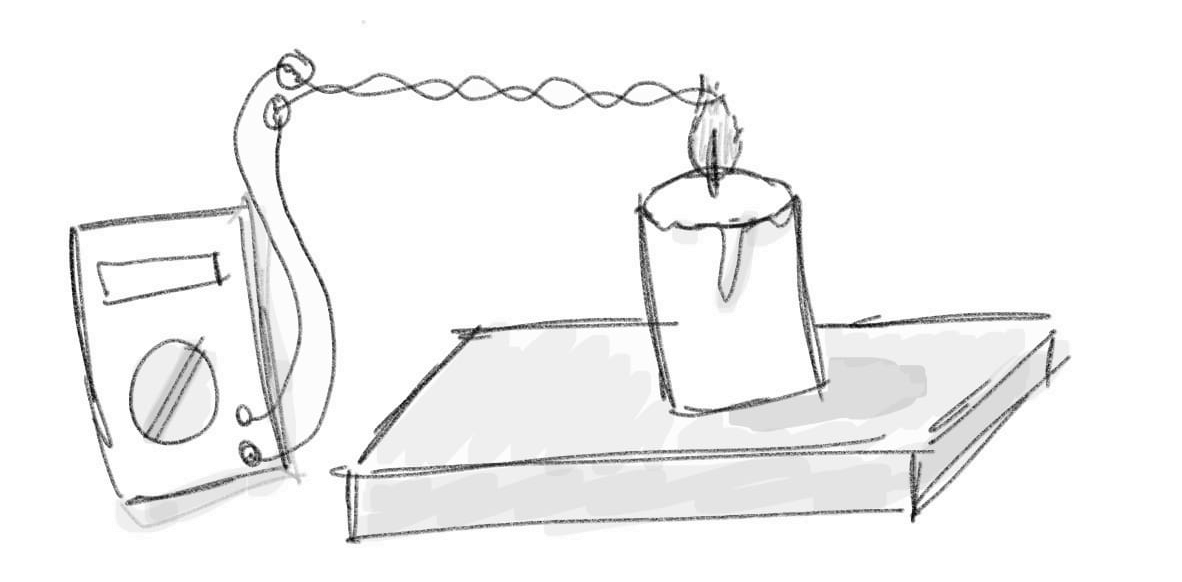
\includegraphics[width=0.75\linewidth]{termopar.png}
    \caption{Termopar}
    \label{fig:enter-label}
\end{figure}\\

Véase en la siguiente tabla los valores registrados.

\begin{table}[h]
\begin{tabular}{l|lll}
                                  & Cobre-Cobre & Cobre-Aluminio & Nicromel-latón \\ \hline
Voltaje $\pm$ 0.05mV & 61.3 mV     & 32.8 mV           & 0.3mV           
\end{tabular}
\end{table}\\

\noindent Este método parece no ser nada efectivo para la producción de energía pues no existe ningún sistema que se vea realmente satisfecho por la diferencia de potencial producida, el gasto en producir esta cantidad de calor (en este caso con 30seg de fuego directo) es muchísimo mayor que lo que conseguiríamos con cualquier otro método menos costoso. En todo caso el termopar cobre-cobre quien resultó ser la mejor combinación podría emplearse en sensores de temperatura de muy bajo consumo o leds.\\

\subsubsection{Celda solar}
Realizamos 10 mediciones durante un minuto del voltaje registrado (1 medición / 6 segundos) obteniendo mediante la desviación standard un valor de $7.\Bar{9}$ V. Esto es un voltaje extremadamente razonable considerando que no necesitamos gastar en combustibles ni reactivos; podremos encender un circuito de leds en serie muchos más potentes que los considerados anteriormente, circuitos de audio, cargar pequeños dispositivos, encender algún motor en protoboard e inclusive un Arduino Nano, Pro Mini, MKR, Due y Lilipad.



\subsubsection{Celda galvánica}
Para el arreglo de la celda galvánica hemos obtenido una cantidad enorme de datos por los cuales a continuación se muestran en una tabla en donde cada celda tiene su valor medido con el multímetro en Volts con incertidumbre $\pm 0.0005V$: \\

\begin{table}[h]
\begin{tabular}{|l|r|r|r|r|r|r|r|r|r|r|}
\hline
  & \multicolumn{1}{l|}{C} & \multicolumn{1}{l|}{Lámina} & \multicolumn{1}{l|}{Al} & \multicolumn{1}{l|}{Ni} & \multicolumn{1}{l|}{Zn} & \multicolumn{1}{l|}{Latón} & \multicolumn{1}{l|}{Sn} & \multicolumn{1}{l|}{Fe} & \multicolumn{1}{l|}{Cu} & \multicolumn{1}{l|}{Mg} \\ \hline
\rowcolor[HTML]{D9D9D9} 
C   & 2.161                       & 1.3                         & 1.231                         & 1.355                       & 1.183                     & 1.747                      & 2.126                       & 1.675                       & 2.046                      & 1.288                         \\ \hline
Lámina   & 1.3                         & 0.42                        & 0.284                         & 0.763                       & 0.487                     & 0.475                      & 0.531                       & 0.343                       & 1.047                      & 0.725                         \\ \hline
\rowcolor[HTML]{D9D9D9} 
Al & 1.231                       & 0.284                       & 1.006                         & 1.189                       & 0.466                     & 1.12                       & 0.37                        & 0.8                         & 0.696                      & 0.534                         \\ \hline
Ni   & 1.355                       & 0.763                       & 1.189                         & 0.298                       & 0.198                     & 0.031                      & 0.759                       & 0.006                       & 0.271                      & 0.002                         \\ \hline
\rowcolor[HTML]{D9D9D9} 
Zn     & 1.183                       & 0.487                       & 0.466                         & 0.198                       & 1.584                     & 1.751                      & 1.682                       & 1.734                       & 1.737                      & 1.512                         \\ \hline
Latón    & 1.747                       & 0.475                       & 1.12                          & 0.031                       & 1.751                     & 1.182                      & 1.403                       & 1.433                       & 1.254                      & 1.362                         \\ \hline
\rowcolor[HTML]{D9D9D9} 
Sn   & 2.126                       & 0.531                       & 0.37                          & 0.759                       & 1.682                     & 1.403                      & 1.918                       & 1.287                       & 1.669                      & 1.916                         \\ \hline
Fe   & 1.675                       & 0.343                       & 0.8                           & 0.006                       & 1.734                     & 1.433                      & 1.287                       & 0.941                       & 0.659                      & 1.465                         \\ \hline
\rowcolor[HTML]{D9D9D9} 
Cu    & 2.046                       & 1.047                       & 0.696                         & 0.271                       & 1.737                     & 1.254                      & 1.669                       & 0.659                       & 1.12                       & 0.909                         \\ \hline
Mg & 1.288                       & 0.725                       & 0.534                         & 0.002                       & 1.512                     & 1.362                      & 1.916                       & 1.465                       & 0.909                      & 2.24                          \\ \hline
\end{tabular}
\end{table}\\

De aquí tenemos que las 3 combinaciones más poderosas son:
\begin{enumerate}
    \item 2.24V – Producido por Mg y Mg.
    \item 2.161V – Producido por C y C.
    \item 2.126V – Producido por C y Sn.
\end{enumerate}

Con este voltaje podemos hacer funcionar microcontroladores de bajo consumo, pantallas lcd pequeñas, lámparas led pequeñas y motores muy chicos.\\

\begin{figure}[h]
    \centering
    \includegraphics[width=0.9\linewidth]{Celda Galvánica.png}
    \caption{Celda galvánica}
    \label{fig:enter-label}
\end{figure}


\section{Conclusiones}

Se ha demostrado que el Generador de Van de Graaff es eficaz en la visualización de fenómenos eléctricos como la polarización y la atracción de objetos cargados. Los resultados confirmaron la capacidad del generador para inducir cargas y provocar efectos visuales notables, como la atracción del confeti y la redistribución de las semillas en el aceite, las cuales ilustraron la presencia y distribución del campo eléctrico.

En cuanto a las fuentes de energía evaluadas, las celdas solares destacaron por su capacidad para generar voltajes significativamente mayores en comparación con las celdas galvánicas y electrolíticas. Esta eficiencia, junto con la ausencia de reactivos costosos, sugiere que las celdas solares son una opción viable y económica para aplicaciones que requieren una fuente de energía estable y sostenible.

Por otro lado, los termopares demostraron ser menos efectivos para la generación de energía, con voltajes generados en el rango de milivoltios, lo que limita su aplicación a sensores de baja potencia o dispositivos específicos como LEDs.

Finalmente, las celdas galvánicas y electrolíticas mostraron una variabilidad en la generación de voltaje dependiendo de los materiales utilizados, con las celdas galvánicas produciendo voltajes más altos en comparación con las electrolíticas. Este resultado indica que, a pesar de su menor costo y complejidad, las celdas galvánicas pueden ser una opción adecuada para aplicaciones que requieren una mayor generación de voltaje.

\newpage
\noindent {\bf Declaración de contribución de los autores}\\ 

Iván Bautista Alvarado$^1$ y Andrés López González$^1$ hemos realizado tanto el apartado escrito como el análisis de manera colectiva siendo una participación del 100\% por parte de ambos y no solo una repartición.\\ 

{\bf Agradecimientos} \\ 

A ese.\\

\begin{figure}[H]
    \centering
    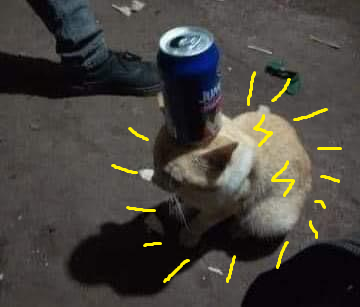
\includegraphics[width=0.5\linewidth]{el.png}
    \caption{Electrogato}
    \label{fig:enter-label}
\end{figure}\\

\begin{thebibliography}{99}

\bibitem{griffiths}
D. J. Griffiths, \textit{Introduction to Electrodynamics}, 3rd ed. Upper Saddle River, NJ, USA: Prentice-Hall, 1999.

\bibitem{jackson}
J. D. Jackson, \textit{Classical Electrodynamics}, 3rd ed. New York, NY, USA: Wiley, 1998.

\bibitem{sadiku}
M. N. O. Sadiku, \textit{Elements of Electromagnetics}, 6th ed. New York, NY, USA: Oxford University Press, 2014.

\bibitem{wangsness}
R. K. Wangsness, \textit{Electromagnetic Fields}, 2nd ed. New York, NY, USA: Wiley, 1986.

\bibitem{zangwill}
A. Zangwill, \textit{Modern Electrodynamics}. Cambridge, UK: Cambridge University Press, 2013.

\bibitem{purcell}
E. M. Purcell and D. J. Morin, \textit{Electricity and Magnetism}, 3rd ed. Cambridge, UK: Cambridge University Press, 2013.

\bibitem{shadowitz}
A. Shadowitz, \textit{The Electromagnetic Field}. Mineola, NY, USA: Dover Publications, 1988.

\bibitem{Feynman}
Feynman, R. P.  \textit{Lectures on physics}. Addison-Wesley. 1964.
\end{thebibliography}

\end{document}